\chapter{Datasets}
\label{ch:data}

The final experiments use two external datasets, RIRD and Wongnai, and one test collection that
we built on top of Wongnai. The datasets play different roles because they contain different
kinds of supervision (Table~\ref{tab:datasets}). Only RIRD can evaluate restaurant ranking. Wongnai
contains real Thai reviews but no labels, so we added our own taste queries and human relevance
labels.

\begin{table}[H]
\centering\small
\caption{The datasets used in the final study.}
\label{tab:datasets}
\begin{tabularx}{\textwidth}{@{}p{2.3cm}LLL@{}}
\toprule
Dataset & Content & Role & Main limitation\\
\midrule
RIRD \citep{rird2023} & 29,168 English reviews of 50 Toronto restaurants; 100 queries judged
against all 50 restaurants by five annotators & Restaurant ranking and explanation evaluation
(RQ1, RQ2) & 50 restaurants in one city; general preferences, not taste\\
Wongnai \citep{wongnai2020} & 40,000 Thai reviews with a 0--4 star rating & Source text for the
Thai track & No restaurant identifiers, no query labels\\
Thai taste test set (this project) & 24 frozen Thai taste queries; 452 query--sentence pairs
labelled 0/1/2 & Sentence retrieval evaluation in Thai (RQ3) & Small; one primary annotator;
sentence level only\\
\bottomrule
\end{tabularx}
\end{table}

\section{RIRD: English reviewed-item retrieval benchmark}
\subsection{Content and structure}
The Reviewed-Item Retrieval Dataset (RIRD) was released by \citet{rird2023}. It contains 29,168
English reviews of 50 restaurants in Toronto. Each review has a restaurant identifier, a star
rating from 1 to 5, the review text, the restaurant categories and a date. The dataset also
contains 100 natural-language queries, for example ``I am on a budget'', ``a bar with a patio'',
``not Thai but Asian'' and ``I am tired so I don't want to wait for seats''. Every query is judged
against every one of the 50 restaurants by five annotators, giving 5,000 query--restaurant
judgements. The queries describe general dining needs (price, occasion, atmosphere, speed,
dietary needs) and include several with explicit negation or exclusion.

\subsection{Relevance labels}
We remove duplicate judgement rows and build two kinds of labels from the five annotator votes.
\emph{Binary} labels use the dataset's aggregated relevance column and are used for MAP, MRR,
precision and recall. \emph{Graded} labels are the number of annotators who marked the pair as
relevant (0 to 5) and are used for nDCG. Because every query is judged against the same 50
restaurants, the judgements are complete: there are no unjudged restaurants, and models can be
compared query by query with paired tests.

\subsection{Exploratory data analysis}
Figure~\ref{fig:rird-eda} summarises the dataset. Three properties shaped the methodology.
\begin{itemize}
  \item \textbf{Uneven review volume (panel a).} Restaurants have between 406 and 2,281 reviews.
  One restaurant has more than five times as many reviews as the smallest ones. This is the
  reason for the volume control described in Chapter~\ref{ch:problem}: every restaurant is also
  evaluated with a random sample of 400 reviews.
  \item \textbf{Varying query difficulty (panel b).} A query has on average 13.5 relevant
  restaurants out of 50, but the number ranges from 1 to 46. Queries with few relevant
  restaurants are much harder, so per-query results vary widely and confidence intervals are
  needed.
  \item \textbf{Long reviews (panel c).} The median review has 94 words and some have several
  hundred. A long review usually discusses many topics, of which only one or two match a query.
  This motivates sentence-level units, which isolate the part of a review that matches.
\end{itemize}
Star ratings are skewed towards 4 and 5 stars (73\% of reviews, panel d). We keep them as
metadata only. A high rating says that a diner was satisfied, not that the restaurant fits a
particular query.

\begin{figure}[H]
\centering
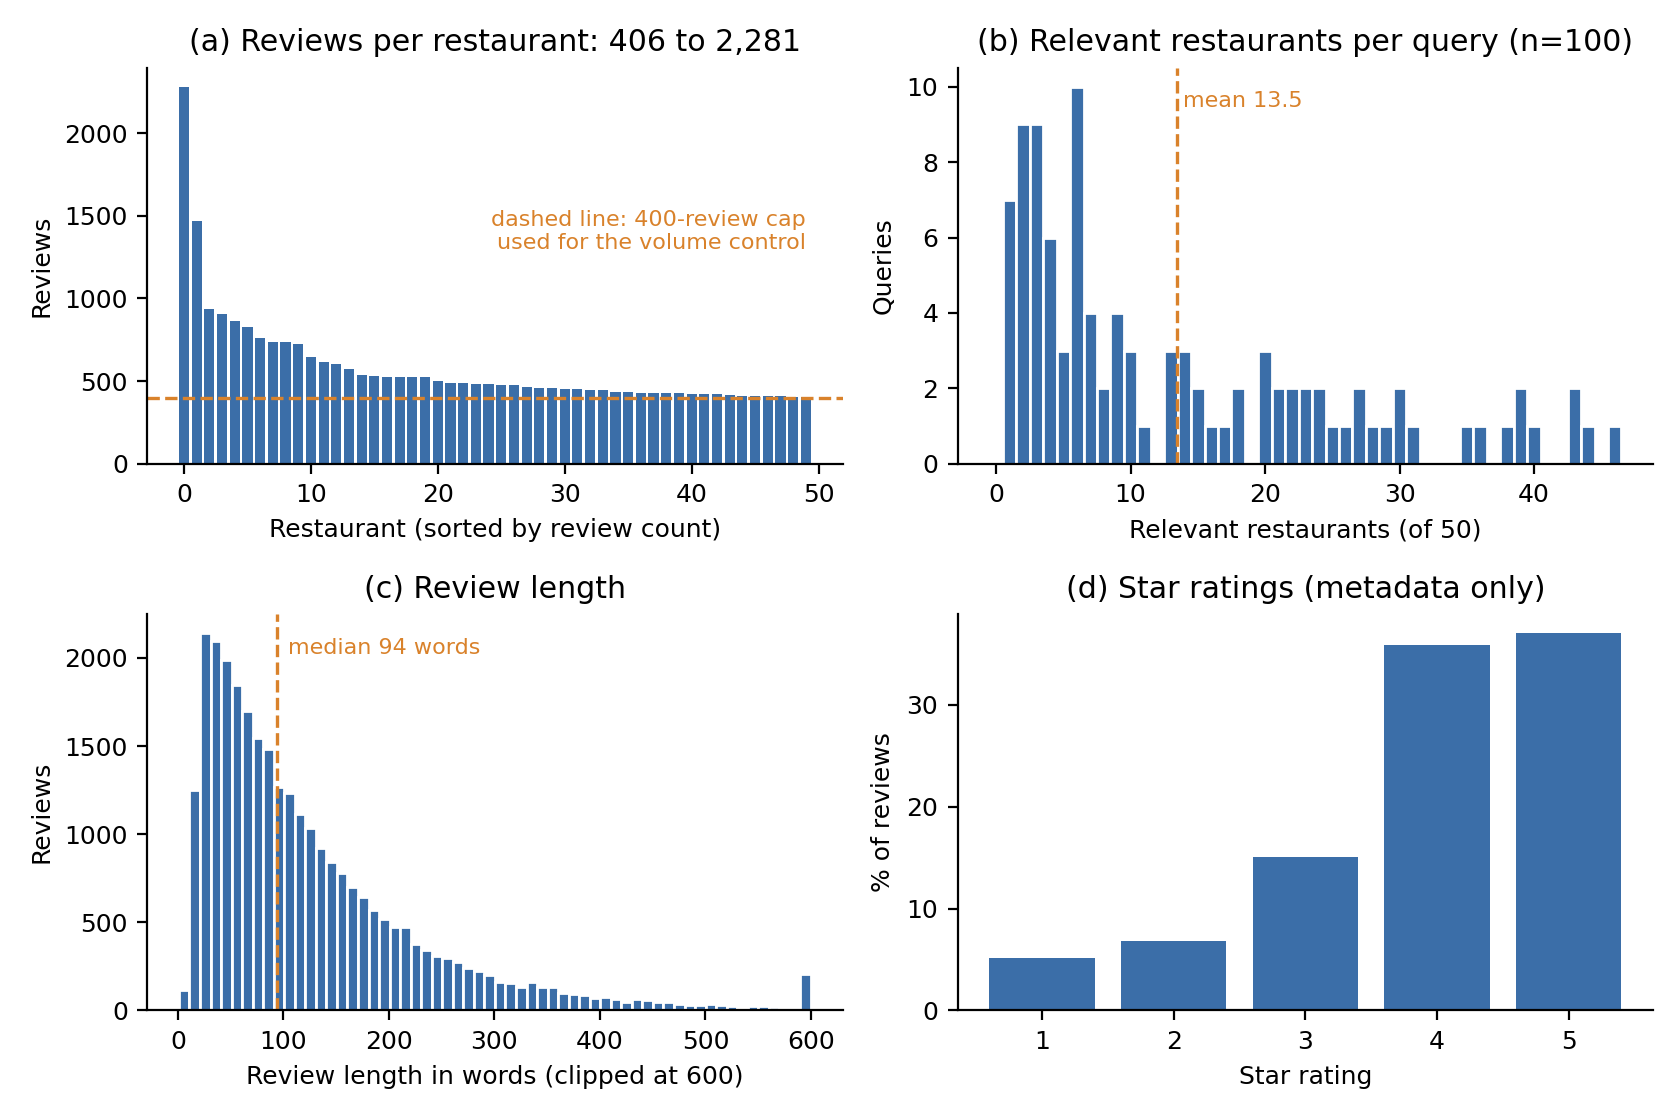
\includegraphics[width=\linewidth]{figures/ch4_rird_eda.png}
\caption{Exploratory analysis of RIRD: (a) reviews per restaurant, with the 400-review cap used
in the volume control; (b) relevant restaurants per query; (c) review length; (d) star
ratings. Data from \citet{rird2023}; figure generated by this project.}
\label{fig:rird-eda}
\end{figure}

\subsection{Pre-processing}
Reviews are split into sentences at sentence-ending punctuation and line breaks, and empty units
are removed. Every sentence keeps its review and restaurant identifiers, so each piece of
evidence can be traced back to its source review. The sentence-level corpus contains 240,660
sentences. For BM25, text is lower-cased and split into word tokens. For the dense model, units
are encoded with \texttt{paraphrase-multilingual-mpnet-base-v2} \citep{reimers2020multilingual}.

\section{Wongnai: Thai restaurant reviews}
\subsection{Content}
Wongnai is a Thai restaurant review platform. We use the public Wongnai review dataset from the
Hugging Face hub \citep{wongnai2020}, which contains 40,000 Thai reviews in its training split
(and 6,203 in a test split that we do not use). Each record has only two fields: the review text
and a star rating from 0 to 4. There is no restaurant name or identifier and no query or
relevance information.

\subsection{Exploratory data analysis}
Figure~\ref{fig:wongnai-eda} shows the star distribution and review length. Ratings are
concentrated at 2 and 3 on the 0--4 scale (77\% of reviews), and the median review is 371
characters long. Reviews are written informally: they mix Thai and English, repeat letters for
emphasis (\thai{เผ็ดดดด}), use slang (\thai{แซ่บ}) and often lack sentence-ending punctuation.
These properties make sentence segmentation harder than in English.

\begin{figure}[H]
\centering
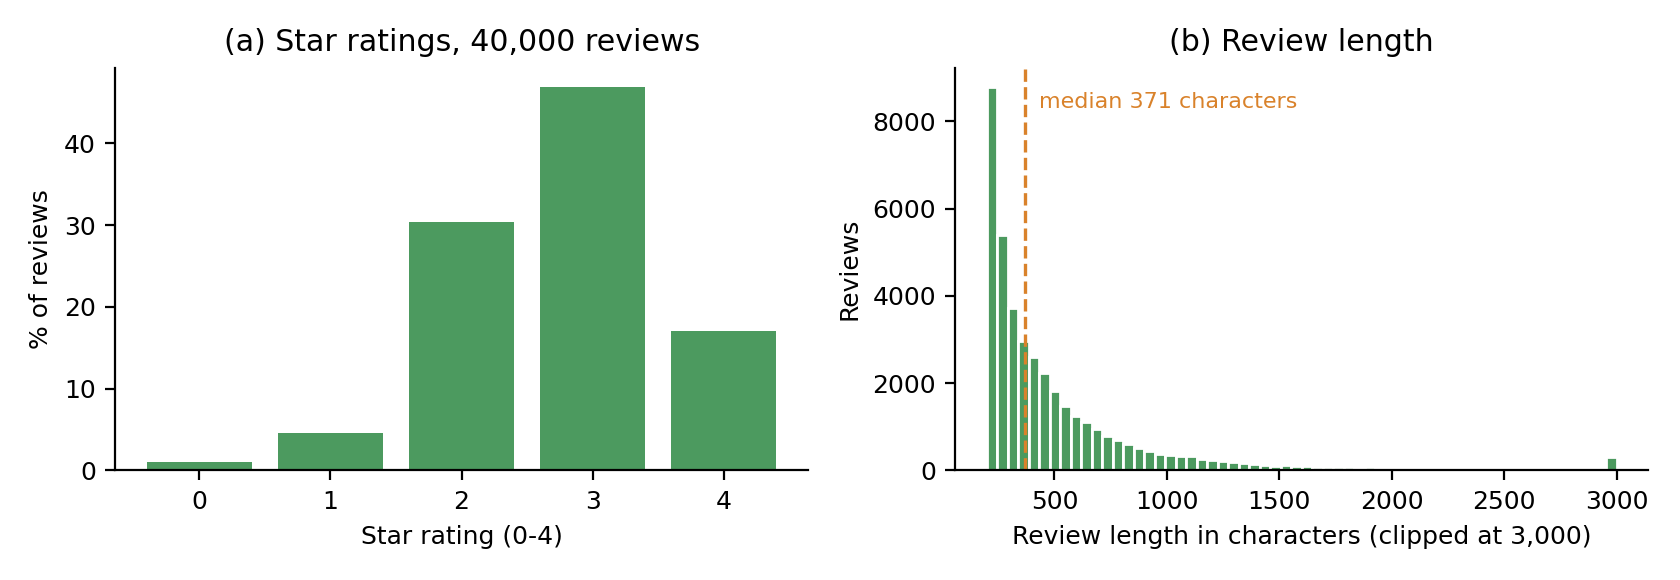
\includegraphics[width=\linewidth]{figures/ch4_wongnai_eda.png}
\caption{Exploratory analysis of the Wongnai training split: (a) star ratings; (b) review length
in characters. Data from \citet{wongnai2020}; figure generated by this project.}
\label{fig:wongnai-eda}
\end{figure}

\subsection{Sampling and pre-processing}
We draw a fixed random sample of 10,000 reviews (seed 42). Each review is split into sentences
with the PyThaiNLP \texttt{crfcut} segmenter \citep{phatthiyaphaibun2023pythainlp}, whitespace is
normalised, and sentences shorter than 15 characters are removed because they are mostly
fragments. The result is a corpus of 93,810 Thai sentences, 9.4 per review on average. For BM25,
sentences are tokenised with the PyThaiNLP \texttt{newmm} word tokeniser and Latin text is
lower-cased. The dense model is the same multilingual encoder used for English.

\section{Thai taste test set}
Wongnai has no relevance labels, so it cannot evaluate retrieval on its own. We therefore built a
small test collection on top of the 10,000-review sample. We followed standard pooled
evaluation: fix the queries first, pool the top results of every system, and have a person label
the pool without knowing which system retrieved each sentence.

\subsection{Queries}
A native Thai speaker in the team wrote 24 Thai taste queries in the style of real requests (Table~\ref{tab:thai-queries}).
They cover ten taste properties and three query types: 11 \emph{single} queries with one
property, 8 \emph{combination} queries with two or three properties, and 5 \emph{negation}
queries such as \thai{ของหวานที่ไม่หวานมาก} (desserts that are not too sweet).
Figure~\ref{fig:thai-testset}a shows the coverage. The queries were frozen on 17 October 2026, before any retrieval results were
inspected. This prevents the queries from being tuned to favour one system.

\begin{table}[H]
\centering\small
\caption{Examples of the 24 frozen Thai taste queries.}
\label{tab:thai-queries}
\begin{tabularx}{\textwidth}{@{}p{1.0cm}p{4.6cm}Lp{1.8cm}@{}}
\toprule
ID & Thai query & English meaning & Type\\
\midrule
T01 & \thai{อยากกินอะไรเปรี้ยวๆ} & I want something sour & single\\
T06 & \thai{ร้านถูกๆ แต่อร่อย} & cheap but tasty place & single\\
T09 & \thai{น้ำซุปหอมสมุนไพร} & broth fragrant with herbs & single\\
T11 & \thai{ต้มยำเปรี้ยวๆ เผ็ดๆ} & sour and spicy tom yum & combination\\
T14 & \thai{แกงกะทิเข้มข้น หวานมัน} & rich, sweet, creamy coconut curry & combination\\
T19 & \thai{อาหารไม่เผ็ด เด็กกินได้} & non-spicy food that children can eat & negation\\
T20 & \thai{ของหวานที่ไม่หวานมาก} & desserts that are not too sweet & negation\\
T22 & \thai{อาหารไม่มัน ไม่เลี่ยน} & food that is not oily or greasy & negation\\
\bottomrule
\end{tabularx}
\end{table}

\subsection{Pooling}
For each query, BM25 and the dense model each retrieve their top 10 sentences from the 93,810.
The union of the two lists forms the judgement pool. The two systems retrieve very different
sentences: on average only 1.2 of their top 10 sentences overlap. The final pool contains 452
unique query--sentence pairs, 18.8 per query on average (between 13 and 20). Because both systems
are judged to depth 10, nDCG@10 and precision@10 can be computed exactly for both. The pool is
not guaranteed to be complete for other systems, so any new system would need its unjudged
sentences labelled before it can be compared.

\subsection{Labelling}
The 452 pairs were shuffled into a blind label sheet that hides the system, rank and score. The
annotation guidelines were written and frozen on 2 November 2026, before labelling began. Each pair is
labelled on a three-point scale:
\begin{description}
  \item[2 (relevant)] the sentence clearly says the food, drink or place has the queried taste,
  at the degree asked, and satisfies every part of the query, including the negation;
  \item[1 (partial)] the taste is weak or hedged, only some parts of a combination are met, or
  the right taste is described for the wrong kind of item;
  \item[0 (not relevant)] the sentence is not about the query, contradicts it (for example
  ``not spicy'' for a spicy query), or uses the query word in an unrelated sense.
\end{description}
The guidelines also define rules for degree words, negation, combinations, sarcasm and
segmentation errors, with worked examples taken from real Wongnai sentences. The label measures
relevance to the query, not sentiment: a complaint that the food was too oily is relevant to a
query asking for oily food.

All 452 pairs were labelled by a native Thai speaker in the team. The result is 184 pairs
labelled 0, 180 labelled 1 and 88 labelled 2 (Figure~\ref{fig:thai-testset}b). One query,
T05 (oily fried food), has no relevant sentence in its pool. Combination queries have the most
partial labels (54\%), because a sentence often matches one taste but not all of them.

To check label consistency, the annotator re-labelled a 60-pair subset by hand in a second
round, following the same frozen guidelines. Agreement with the first round is high: 90\% exact
agreement, Cohen's $\kappa = 0.837$ \citep{cohen1960kappa} and linearly weighted
$\kappa = 0.869$. Because both rounds were labelled by the same person, this measures the
consistency of the labels rather than agreement between two different annotators.

\begin{figure}[H]
\centering
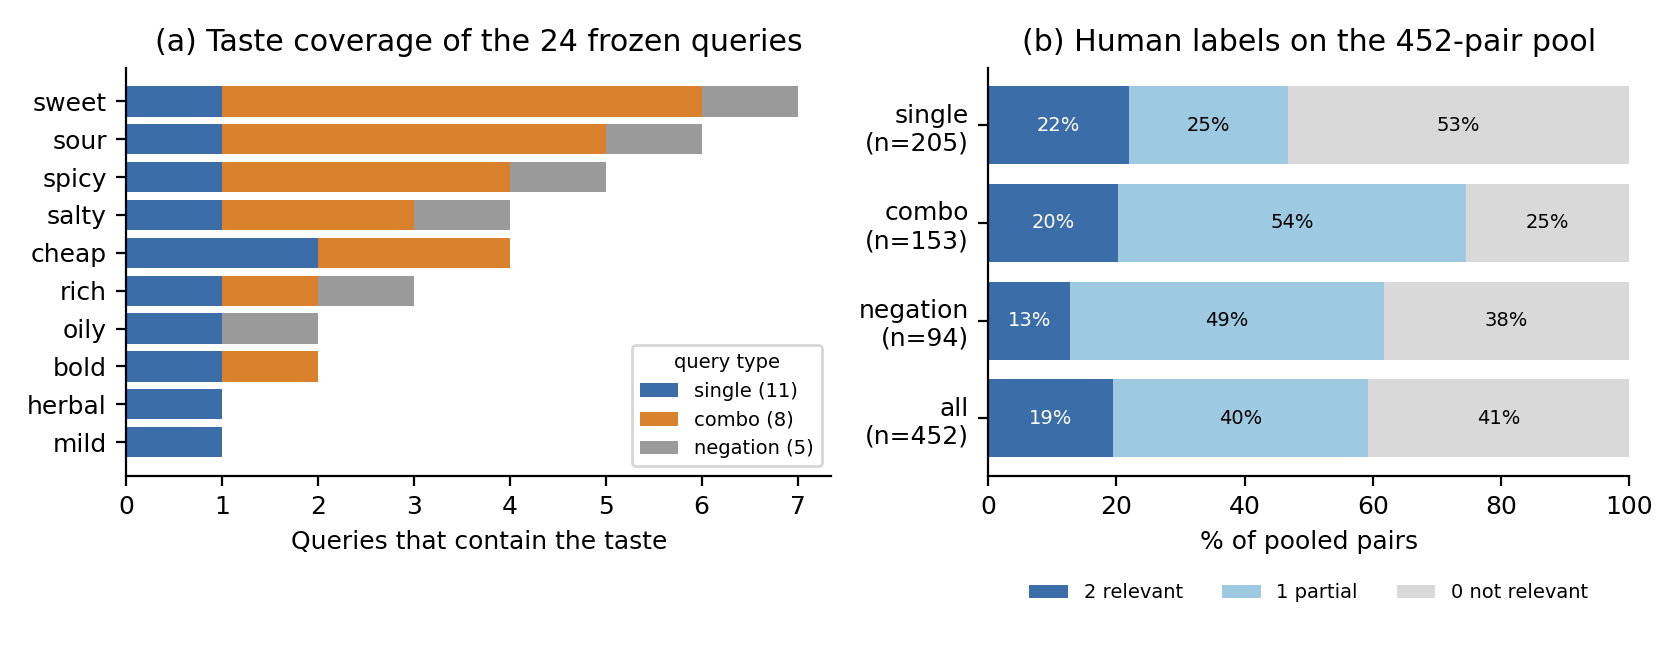
\includegraphics[width=\linewidth]{figures/ch4_thai_testset.png}
\caption{The Thai taste test set: (a) taste properties covered by the 24 queries, by query type;
(b) distribution of human labels in the 452-pair pool, by query type. Generated by this project
from Wongnai sentences \citep{wongnai2020}.}
\label{fig:thai-testset}
\end{figure}

\subsection{Star ratings are not relevance labels}
The labelled pool also shows why Wongnai star ratings cannot replace query labels. The rank
correlation between a sentence's review star rating and its relevance label is weak (Spearman
$\rho = 0.10$). Sentences from 4-star reviews are labelled not relevant 31\% of the time, and
sentences from 1-star reviews are labelled relevant 23\% of the time (5 of 22). A rating describes the
whole visit, while the label describes whether one sentence answers one request.

\section{Datasets considered but not used}
The proposal also considered the Thailand Foods dataset \citep{thailandfoods} and the Thai
subset of M-ABSA \citep{mabsa}. Neither provides the query--item relevance structure needed for
the evaluation. Thailand Foods lists dish names and food attributes; it could support a future
food-term dictionary or query normalisation, but it has no review text, restaurant identifiers
or relevance judgements. M-ABSA provides aspect--sentiment labels, which are useful for Thai
sentiment research, but they do not say whether a sentence satisfies a search query. Using either
resource as ground truth would mean evaluating the system against features designed by the
authors themselves, so both were left out.

\section{Data provenance and limitations}
RIRD and Wongnai are public datasets, used here for academic research and cited in the
bibliography. All figures in this report are generated by the project from these datasets or
from our own experiment outputs; none is copied from an external publication. Review text is
subjective and may be outdated or contradictory, so the system presents it as evidence rather
than fact. RIRD covers only 50 restaurants in one city. Wongnai cannot support restaurant-level
evaluation, and the Thai test set is small (24 queries) with one primary annotator, which limits
the statistical power of the Thai comparison.
